\documentclass[aspectratio=43]{beamer}

%%%%%%%%%%%%%%%%%%%%%%%%%%%%%%%%%%%%%%%%%%%%%%%%%%%%%%%%%%%%%%%%%%%%
% über aspectratio kann das Format eingestellt werden. Der Default
% wert ist 43 (4:3, 128mm:96mm). Andere Möglichkeiten sind
% 32 (3:2, 135mm:90mm)
% 54 (5:4, 125mm:100mm)
% 149 (14:9, 14cm:9cm)
% 169 (16:9, 16cm:9cm)
% 1610 (16:10, 16cm:10cm)
% 141 (1.41:1, 148.5mm:105mm, Seitenverhältnis wie bei DIN-A)
%%%%%%%%%%%%%%%%%%%%%%%%%%%%%%%%%%%%%%%%%%%%%%%%%%%%%%%%%%%%%%%%%%%%


\usepackage[T1]{fontenc}
\usepackage[utf8x]{inputenc}
\usepackage[ibycus,ngerman]{babel}
\usepackage{amsfonts,amsmath,amssymb,amsthm}
\usepackage{csquotes}

\usepackage{hyperref}

\DeclareMathOperator{\atan}{atan2}




\usetheme[komms=false]{fbmathematik}

%%%%%%%%%%%%%%%%%%%%%%%%%%%%%%%%%%%%%%%%%%%%%%%%%%%%%%%%%%%
% Schriftfarben:
% tuklblau, tuklrot, warmgrau, kaltgrau;
% abgeschwächte Töne für die obigen Farben und schwarz:
% z.B. tuklblau7 für 70% tuklblau, warmgrau2 für 20%
% warmgrau oder schwarz6 für 60% schwarz,
% jeweils in den Schritten 10%, 20%, 40%, 60%, 70%, 80%;
% violette Schriftfarbe (Felix-Klein) hat den Namen fkz1
% hellviolette FKZ-Variante hat den Namen fkz2;
% KOMMS: kommsblau, kommsgruen, kommsgrau, kommsblaugrau
%%%%%%%%%%%%%%%%%%%%%%%%%%%%%%%%%%%%%%%%%%%%%%%%%%%%%%%%%%%



\title{Immer der Sonn' entgegen}
\subtitle{1. Zwischenbericht}
\author{Dominik Bendle \and Melissa Hasel \and Thomas Hofmann}
\date{\today}
\institute{TU Kaiserslautern}

\begin{document}

\begin{frame}[plain]

    %\maketitle
    \Titel{logo}

\end{frame}

\begin{frame}
    \frametitle{Ideales Modell: Ausgangspunkt}
    \begin{itemize}
        \item Erde ist im Ursprung zentrierte Kugel
        \item Annahme: Sonne umläuft Erde in ebener Kreisbahn $\rightarrow$
        \item[]$\rightarrow$ skalierter Einheitskreis in der $xy$-Ebene
        \item dabei: konstante Geschwindigkeit mit Umlaufperiode von einem Jahr
        \item geneigte Erdachse gegeben durch Gerade, die durch Ursprung läuft und in
            $xz$-Ebene liegt
        \item Konstanten:
            \begin{itemize}
                \item Entfernung Sonne--Erde: $d_S = 149000000000\,\mathrm m$.
                \item[]$\rightarrow$ Etwaiges Mittel der echten Distanzen
                \item Radius der Erde: $r_E = 6371000\,\mathrm m$
                \item Neigung der Erdachse: Winkel zwischen Erdachse und $z$-Achse im
                    Koordinatensystem: $\alpha_E = 23{,}4^\circ \approx 0{,}13\pi$
            \end{itemize}
    \end{itemize}
\end{frame}

\begin{frame}
    \frametitle{Umlaufmodell bis jetzt:}
    \begin{itemize}
        \item Zum Zeitpunkt $t_0$ sollte sich die Sonne am Punkt $d_S\cdot(1,0,0)^T$
            befinden.
        \item[]$\rightarrow$ 20.\ Juni 12 Uhr: $t_0 = 172{,}5\cdot1440 \,\mathrm{min}$.
        \item All dies liefert folgende Parametrisierung der Sonnenposition
            \begin{equation*}
                \gamma_S(t) = d_S \cdot
                \begin{pmatrix}
                    \cos(\omega (t - t_0)) \\
                    \sin(\omega (t - t_0)) \\
                    0
                \end{pmatrix},
            \end{equation*}
            wobei $\omega = \frac{2\pi}{365\cdot1440\,\mathrm{min}}$
    \end{itemize}
\end{frame}

\begin{frame}
    \frametitle{Erde fixieren}
    \begin{itemize}
        \item In diesem Modell rotiert die Erde noch!
        \item Erster Schritt: Erdachse auf $z$-Achse drehen: Brauchen per Konstruktion
            Dreh-Matrix um $y$-Achse:
            \begin{equation*}
                R_y(\alpha) =
                \begin{pmatrix}
                    \cos(\alpha) & 0 & \sin(\alpha) \\
                    0 & 1 & 0 \\
                    -\sin(\alpha) & 0 & \cos(\alpha)
                \end{pmatrix}
            \end{equation*}
        \item Anschließend: Eigenrotation der Erde durch Rotationsmatrix um $z$-Achse
            ausgleichen:
            \begin{equation*}
                R_z(\alpha) =
                \begin{pmatrix}
                    \cos(\alpha) & \sin(\alpha) & 0 \\
                    -\sin(\alpha) & \cos(\alpha) & 0 \\
                    0 & 0 & 1
                \end{pmatrix}
            \end{equation*}
    \end{itemize}
\end{frame}

\begin{frame}
    \frametitle{Fertiges Umlaufmodell}
    \begin{itemize}
        \item Zuerst um $\alpha_E$ drehen, um Erdachse zu \enquote{begradigen}
        \item Dann in Abhängigkeit von der Zeit um $z$-Achse drehen:
        \item Somit:
            \begin{equation*}
                \tilde \gamma_S(t) = R_z(-\omega_E\cdot (t - t_0)) \cdot R_y(-\alpha_E) \cdot
                \gamma_S(t)
            \end{equation*}
            wobei $\omega_E=\frac{2\pi}{1440\,\mathrm{min}}$.
        \item Somit sind die Koordinaten der Erdkugel invariant in der Zeit
    \end{itemize}
\end{frame}

\begin{frame}
    \frametitle{Erstes Wandermodell}
    \begin{itemize}
        \item Können nun für gegebene Position auf Erde zu gegebener Zeit (in Minuten seit Neujahr)
            Sonnenposition bestimmen
        \item[]$\rightarrow$ Laufrichtung beim Verfolgen der Sonne
        \item benötigen folgende Daten
            \begin{itemize}
                \item $p=(x_p, y_p, z_p)^T$ Punkt auf der Erdoberfläche ($\|p\|_2 =
                    r_E$)
                \item $t$ Zeit in min
                \item $\Delta_t$ Zeit, für die nach ermittelter Laufrichtung geradeaus
                    gelaufen werden soll in min
                \item[]$\rightarrow$ Approximation der Laufkurve durch Polygonzug
                \item $v$ Laufgeschwindigkeit in m$/$min
            \end{itemize}
        \item suchen also neue Position $p_{\text{neu}}$
    \end{itemize}
\end{frame}

\begin{frame}
    \frametitle{Erstes Wandermodell}
    \begin{itemize}
        \item da wir von Fortbewegung zu Fuß ausgehen, ist die relevante Kugeloberfläche
            für hinreichend kleine $\Delta_t$ eben, also bewegen wir uns der auf der
            Tangentialebene in $p$ und projizieren dann
        \item[]$\rightarrow$ hat auf Kugel Normalenvektor $p$
        \item setze $v_S = \gamma(t) - p$, die \enquote{Blickrichtung} zur Sonne von
            $p$ aus, dann ergibt sich Projektion von $p_S$ auf Tangentialebene als
            \begin{equation*}
                v_r = v_S - \left( v_S \cdot \frac1{\|p\|_2}p \right) \cdot
                \frac1{\|p\|_2} p
            \end{equation*}
    \end{itemize}
\end{frame}

\begin{frame}
    \frametitle{Fortbewegen \& Normieren}
    \begin{itemize}
        \item somit gehen wir in Richtung der Sonne:
            \begin{equation*}
                \tilde p = p + \frac{\Delta_t*v}{\|v_r\|}v_r
            \end{equation*}
        \item Durch Normieren oder Rückskalieren auf die Kugel erhalten wir unsere neue
            Position:
            \begin{equation*}
                p_{\text{neu}} = \frac{r_E}{\|\tilde p\|}\tilde p
            \end{equation*}
    \end{itemize}
\end{frame}

\begin{frame}
    \frametitle{Berücksichtigung von Sonnenunter- \& Aufgang}
    \begin{itemize}
        \item zwar theoretisch möglich, wollen uns aber nicht mehr bewegen, wenn Sonne
            nicht mehr sichtbar
        \item[]$\rightarrow$ wenn Sonne unter Horizont
        \item[]$\rightarrow$ im Ideallmodell: $\measuredangle(p, v_S) > 90^\circ$
        \item wie Winkel zwischen Vektoren berechnen? Verwenden:
            \begin{equation*}
                a \times b = \|a\| \|b\| \sin\alpha \cdot n,\quad
                a \cdot b = \|a\| \|b\| \cos\alpha
            \end{equation*} falls $\alpha = \measuredangle(a, b)$, also $\tan\alpha =
            \frac{\|a\times b\|}{a\cdot b}$
        \item atan2 liefert Fallunterscheidungen bei Umkehrung mit: $\alpha =
            \atan(\|a\times b\|, a\cdot b)$.
    \end{itemize}
\end{frame}

\begin{frame}
    \frametitle{Pfadbeispiele}
    \begin{figure}[t]
        \centering
        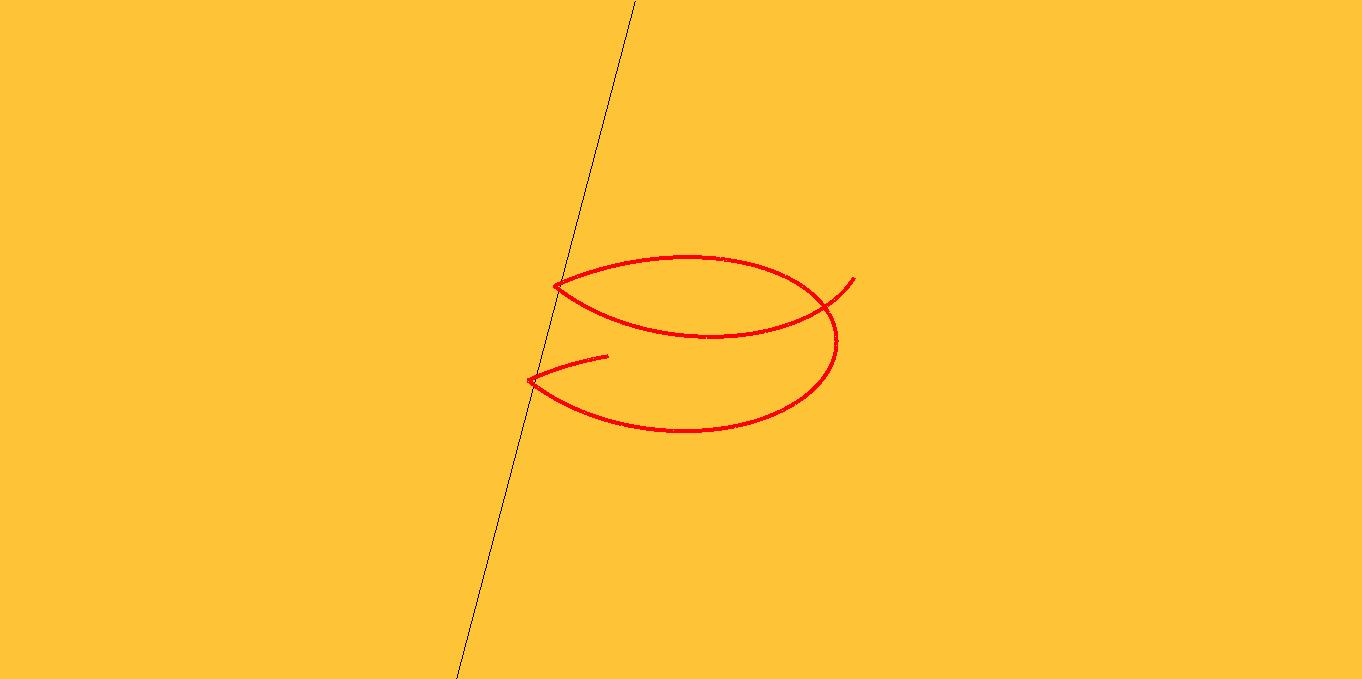
\includegraphics[width=0.9\textwidth]{bilder/d172lon7lat47.jpg}
        \caption{ca. 1,5 Tage Laufen: 47$^\circ$ O, $7^\circ$ N, Beginn 20. Juni}
    \end{figure}
\end{frame}

\end{document}
